\documentclass[a4paper,12pt]{report}
\usepackage[utf8]{inputenc}
\usepackage{graphicx}
\usepackage{hyperref}
\usepackage{textcomp}
\usepackage{mathtools}

\begin{document}

\chapter{}
\section{Theory recap: flanger with feedback}
Flanger is a delay-based effect. So, we started from the implementation of the \textbf{Delay Line}, considering that the amount of the delay varies over time, under the control of a separate \textbf{Low-Frequency Oscillator} \textbf{(LFO)}. Moreover, adding a \textbf{feedback control}, the output of the delay line is routed back to its input. %This causes the sound to repeat continuously, and assuming a feedback gain less than 1, the echoes will become quieter each time. Though the echoes are theoretically repeated forever, they will eventually become so quiet as to be below the ambient noise in the system and thus be inaudible.
\\In the picture below a block diagram of a flanger with feedback unit is shown:
\begin{figure}[h]
\centering
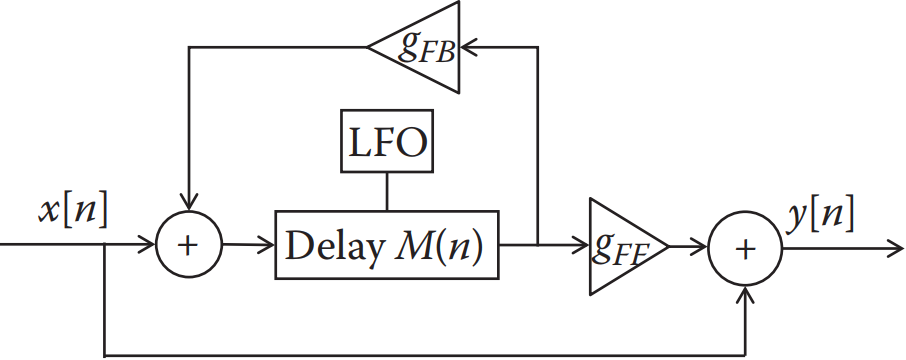
\includegraphics[scale=.45]{db_flanger.png}
\caption{Flanger with feedback}
\end{figure}
\\As we can see from the block diagram, we have two gains, $\textit{g}_{FB}$, which is the feedback gain, and $\textit{g}_{FF}$, the gain related to the output of the delay line. If $\textit{g}_{FB}<1$, the delayed copies of the sound will gradually decay, where a gain of 1 or more means they will grow indefinitely.
So, the input/output relation for the flanger with feedback can be expressed in the time domain as:
\[ y[n] = x[n]+ g_{FF}d[n]\] where $d[n]=x[n-M[n]]+g_{FB}d[n-M[n]] $ is the output of the delay line. $M[n]$ expresses the delay length over a sample $n$. There are different $M$ functions, depending on the particular waveform we are using. Generally, we can describe $M$ through the following parameters: 
\begin{itemize}
\item[\textperiodcentered] $M_{0}$ (in samples), the delay given by the delay control;
\item[\textperiodcentered] $M_{W}$ (in samples), the delay given by the sweep width control; 
\item[\textperiodcentered] $\phi$, the phase of the waveform (in rad).
\end{itemize}
For our plugin we are going to use the following waveforms, with $\phi \in [0,1]$:
\begin{itemize}
\item[\textperiodcentered] Sine: \[ M(\phi) = M_{0}+M_{W}(\frac{1}{2}+\frac{1}{2}\sin(2\pi \phi))\] 
\item[\textperiodcentered] Triangle:
  \begin{equation}
    M(\phi) =
    \begin{cases*}
      M_{0} + M_{W}(\frac{1}{2}+2\phi) & if $0\leq \phi<\frac{1}{2}$ \\
      M_{0} + M_{W}(1-2(\phi-1/4)) & if $\frac{1}{2}\leq \phi<\frac{3}{4}$ \\
      M_{0} + 2M_{W}(\phi-\frac{3}{4}) & if $\frac{3}{4}\leq \phi\leq 1$
    \end{cases*}
\end{equation}
\item[\textperiodcentered] Sawtooth:
  \begin{equation}
    M(\phi) =
    \begin{cases*}
      M_{0} + M_{W}(\frac{1}{2}+\phi) & if $\phi\leq \frac{1}{2}$\\
      M_{0} + M_{W}(\phi-\frac{1}{2}) & if $\frac{1}{2}<\phi\leq 1$
    \end{cases*}
\end{equation}
\end{itemize}
\end{document}
